%% 
%% Copyright 2007-2020 Elsevier Ltd
%% 
%% This file is part of the 'Elsarticle Bundle'.
%% ---------------------------------------------
%% 
%% It may be distributed under the conditions of the LaTeX Project Public
%% License, either version 1.2 of this license or (at your option) any
%% later version.  The latest version of this license is in
%%    http://www.latex-project.org/lppl.txt
%% and version 1.2 or later is part of all distributions of LaTeX
%% version 1999/12/01 or later.
%% 
%% The list of all files belonging to the 'Elsarticle Bundle' is
%% given in the file `manifest.txt'.
%% 
%% Template article for Elsevier's document class `elsarticle'
%% with harvard style bibliographic references

\documentclass[final,5p,times,twocolumn]{elsarticle}

%% Use the options 1p,twocolumn; 3p; 3p,twocolumn; 5p; or 5p,twocolumn
%% for a journal layout:
%% \documentclass[final,1p,times]{elsarticle}
%% \documentclass[final,1p,times,twocolumn]{elsarticle}
%% \documentclass[final,3p,times]{elsarticle}
%% \documentclass[final,3p,times,twocolumn]{elsarticle}
%% \documentclass[final,5p,times]{elsarticle}
%% \documentclass[final,5p,times,twocolumn]{elsarticle}

%% For including figures, graphicx.sty has been loaded in
%% elsarticle.cls. If you prefer to use the old commands
%% please give \usepackage{epsfig}

%% The amssymb package provides various useful mathematical symbols
\usepackage[utf8]{inputenc}
\usepackage{textcomp}

\usepackage{graphicx}
\usepackage{float}

\usepackage{times}
\usepackage{color}
\usepackage{xcolor}
\usepackage{natbib} 
\usepackage{enumerate}
\usepackage{caption}
%\usepackage[separator = {;}]{credits}
\usepackage{lscape}
\usepackage{subcaption}
\usepackage{wrapfig}
\usepackage{orcidlink}
\usepackage{amssymb}
\usepackage{amsthm}
\usepackage{enumitem}
\usepackage{hyperref}
\hypersetup{colorlinks=true,
	 citecolor=cyan,
	 pdfauthor=cyan,
	 linkcolor=cyan}


\journal{Journal of Space Safety Engineering}

\begin{document}

\begin{frontmatter}

\title{Analysis of ETRSS-1 on-orbit performance and anomaly management}
%\tnotetext[t1]{This document is the results of the research project funded by the Aerospace System and Control Lab, ASCL}

\author[1]{Gadisa Dianol\corref{cor1}}
\fnref{fn1}
\ead{gdina@kaist.ac.kr}
%\credit{Conceptualization,  Writing - Original draft, Methodology, Data curation, Writing -review and editing, and Visualization }
%\author[1]{Hyochoong Bang\fnref{fn2}}
%\ead{hcbnag@kaist.ac.kr}
%\credit{Reviewing and editing,  Supervision, and Funding acquisition}
\cortext[cor1]{Corresponding author}
\fntext[fn1]{Researcher at Aerospace System and Control Lab, Department Aerospace engineering, KAIST, 34141, Republic of Korea}
%\fntext[fn2]{Professor of Aerospace Engineering at Korean Advanced Institute of Science and Technology (KAIST), Daejeon, 34141, Republic of Korea}

\affiliation[1]{organization={Aerospace System and Control Lab, Korean Advanced Institute of Science and Technology, KAIST},%Department and Organization
            addressline={291}, 
            city={Daejoen},
            postcode={34141}, 
            country={Republic of Korea}}
%\affiliation[2]{}
\begin{abstract}
The Ethiopian remote sensing micro-satellite, weighing 65 kilograms, was successfully launched into sun-synchronous orbit at an altitude of 628 kilometers in 2019. The satellite has a three-year lifespan and will spontaneously decay after 25 years.  The ETRSS-1 satellite's on-orbit performance and anomaly management are critical for establishing its operating capabilities and ensuring mission success. This study aims to provide an overview of the ETRSS-1 satellite system, including its subsystems such as AOCS, communication, on-board computer, power supply, and thermal control system, along with the hardware utilized during their development, as well evaluate their on-orbit performance and identify any anomalies or deviations from expected behavior. Additionally, the anomaly management technique utilized by mission operators to identify and handle any unexpected events or failures is discussed. The spacecraft's electro-optical multi-spectral camera and its capacity to capture remote sensing data while adhering to appropriate operational parameters, as well as its imaging mission approaches, might also be examined.The spacecraft's electro-optical multi-spectral camera, its ability to capture remote sensing data while adhering to suitable operational limits, and its imaging mission techniques might all be investigated.  Overall, this study contributes to our understanding of the ETRSS-1 satellite's on-orbit behavior, paving the way for future satellite mission planning and anomaly detection improvements in operating processes and respond techniques.
\end{abstract}

%%Research highlights
%\begin{highlights}
%	\item Technical parameters of the ETRSS-1 satellite system
%	\item The ETRSS-1 spacecraft platform bus
%	\item The AOCS on the ETRSS-1 satellite operate in six modes
%	\item  Malfunctions are classified into four major categories based on their impact on the ETRSS-1 satellite
%	\item The ETRSS-1 optical camera payload is made up of two major parts
%\end{highlights}

\begin{keyword}
	Attitude \sep Anomaly \sep Fault detcetion \sep Microsatellite \sep Mult-spectral \sep SSO \sep Workmode

\end{keyword}
\end{frontmatter}


%% main text
\section{Introduction}
\label{}
The Ethiopian remote sensing microsatellite, weighing 65 kilograms, was successfully launched into space in December 2019 from the Taiyuan launch facility with the mission of providing earth imagery data to address Ethiopian climate change and earth-related issues such as water resources, desertification, vegetation, and other periodic observations, as well as the detection and assessment of natural disasters caused by climate change.  The satellite is controlled from a sun-synchronous orbit at an altitude of 628 kilometers by a ground control station on Mount Entoto. Furthermore, a multispectral Ethiopian remote sensing satellite was made up of two distinct modules: the satellite bus module (platform) and the payload (instrument module), as shown in Fig.1a. The ETRSS-1 platform module comprises six key subsystems, while the payload consists of a multispectral camera and a data transmission system that provides imagery data, as detailed in detail in section 2. The key technical parameters of the ETRSS-1 satellite system are listed in Table 1. \\
\begin{table}[!hb]
	\small
	\caption{Key technical parameters of ETRSS-1} % title of Table
	\centering % used for centering table
	\scalebox{0.8}{
	\begin{tabular}{c c } % centered columns (4 columns)
		\hline\hline %inserts double horizontal lines
		Item name& Designed technical\# parameters\\ [0.5ex] % inserts table
		%heading
		\hline % inserts single horizontal line
		Mass & total mass 65kg \\ % inserting body of the table
		Sun-synchronous orbit & Altitude 628.610 km \\
		Attitude and orbit control system & 3-axis stabilized, zero-momentum control;\\
		& pointing accuracy: 0.1$^{\circ}$/s (3$\sigma$, 3axis in normal mode);\\
		& pointing stability: 0.01$^{\circ}$/s (3$\sigma$, 3-axis);\\
		& attitude determination accuracy: 0.05$^{\circ}$ (3$\sigma$, 3-axis);\\
		& attitude maneuver: $\pm$ 35$^{\circ}$ (along roll axis);\\
		& maneuver capability: 30$^{\circ}$/70s\\
		Telemetry and telecommand & USB + GPS\\
		Power supply system & output poser of solar array be more than 150 W (EOL)\\
		& Li-ion batter capacity: 20Ah\\
		Multi-spectral camera & type: push broom imaging\\
		& B1/blue: 0.45$\mu$m $\thicksim$ 0.52$\mu$m, B2/green: 0.52$\mu$m $\thicksim$ 0.59$\mu$m,\\
		& B3/re: 0.63$\mu$m $\thicksim$ 0.69$\mu$m, B4/NIR: 0.77$\mu$m $\thicksim$ 0.89$\mu$m,\\
		& ground sampling distance: $\leq$ 15m at 645km,\\
		& swath: $\geq$ 60km at 645km\\
		Data transmission system & frequency band: X-band,\\
		& storage capacity: 128 Gbits,\\
		& down-link data rate: 100 Mbps\\
		Life/reliability & more than 2 years /$\geq$ 0.6 \\ [1ex] % [1ex] adds vertical space
		\hline %inserts single line
	\end{tabular}
}
	\label{table:nonlin} % is used to refer this table in the text
\end{table}
\begin{figure*}
	\begin{subfigure}{.5\textwidth}
		\centering
		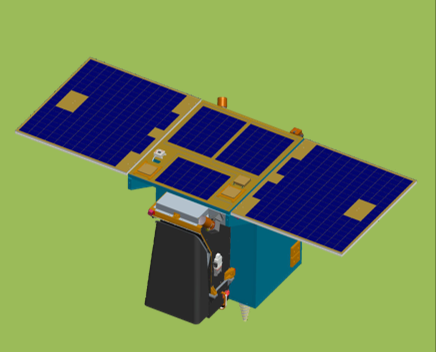
\includegraphics[width=.65\linewidth]{image/ETRSS-1}
		\caption{Ethiopian remote sensing satellite}
	\end{subfigure}
	\begin{subfigure}{.5\textwidth}
		\centering
		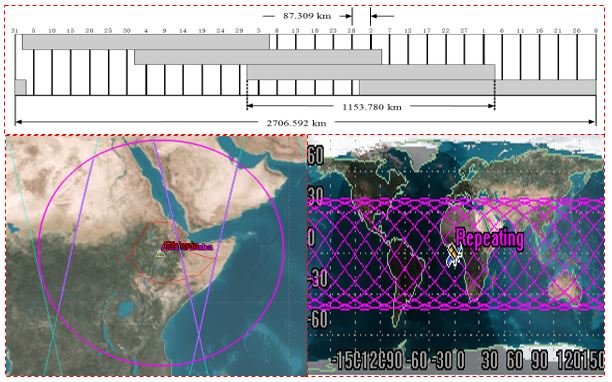
\includegraphics[width=.85\linewidth]{image/Etrss-coverage.JPG}
		\caption{ETRSS-1 coverage}
	\end{subfigure}
	\caption{ETRSS-1 satellite and its coverage (Credit: DFH SATELLITE Co.,Ltd)}
\end{figure*}
The vast majority of remote sensing satellite platforms are in near-polar orbits, which means they travel north on one side of the Earth and then south on the other, a process known as ascending and descending, in order to record reflected or emitted (e.g., thermal) radiation from the surface using on-board sensors. Furthermore, Earth observation satellite missions frequently require constant solar illumination, the same ground resolution, and short repeat cycles, leading to the design of a repeat Sun-Synchronous Orbit (SSO) as the most appropriate, allowing observation of a given region of the Earth at the same local time after a time interval \cite{Luo2017ANT}. In this regard, ETRSS-1 is collecting remote sensing imaging data from a sun-synchronous orbit with a local time of the descending node of 10:30AM, a revising period of 4 days, and a ground sampling distance more than 15 meters. Table 2, describes ETRSS-1's Keplerian orbital parameters, which are derived from the satellite's real-time orbital tracking and are used to describe the shape and orientation of the satellite's orbit and position.
As ETRSS-1 orbits the Earth, its payload sensor footprint covers a portion of the planet's ground surface, focusing on East African countries (Fig.1b) in an 87.309-kilometer-wide equatorial swath with each successive pass, the apparent movement allowing the satellite swath to cover a new area, and its camera coverage reaches 1153.780km with 38$^{\circ}$ rolling maneuvering and 4 days revisiting periods. The access times between ETRSS-1 and ground control station during one day are 2 $\thicksim$ 4; the maximum time is 10.59 min for accessing; and the maximum time is 33.33 min for all accessing in one day.
\begin{table}[ht]
	\small
	\caption{Orbital parameters of ETRSS-1} % title of Table
	\centering % used for centering table
	\scalebox{0.7}{
	\begin{tabular}{c c c c} % centered columns (4 columns)
		\hline\hline %inserts double horizontal lines
		Orbit element representation& Elemental name& \# Parameter \\ [0.5ex] % inserts table
		%heading
		\hline % inserts single horizontal line
		a & Semi-major axis & 6999.614 km \\ % inserting body of the table
		e & Eccentricity& .0016456 \\
		i & Inclination & 97.8963$^{\circ}$ \\
		$\Omega$& Right Ascension of  Ascending Node (RAAN)& 289.4525$^{\circ}$\\
		$\omega$& Argument of Perigee & 67.9288$^{\circ}$\\
		f & True anomaly & 292.3649$^{\circ}$\\
		h & Altitude & 628.610 km \\
		LTDN & Local Time of Descending Node& 13:30 PM \\
		- & Flight Circles per Day & 14.806\\
		- & Revisiting periods & 4 days\\
		$\tau$ & orbital period (min) & 97.134 \\ [1ex] % [1ex] adds vertical space
		\hline %inserts single line
	\end{tabular}
	}
	\label{table:nonlin} % is used to refer this table in the text
\end{table}
This study aims to provide an overview of the anomaly management procedure used by mission operators to identify and resolve any unexpected events or malfunctions.  Additionally, the spacecraft's electro-optical multispectral camera and its capacity to capture remote sensing data while adhering to appropriate operational parameters, as well as its imaging mission techniques, might also be examined. Overall, the study contributes to a better understanding of the ETRSS-1 satellite's on-orbit behavior, allowing improvements in operational procedures, anomaly response strategies,  future satellite mission planning and anomaly detection.
\section{Ethiopian remote sensing satellite subsystems}
The Ethiopian remote sensing satellite was developed based on the standardized satellite platform of CAST \cite{zhu2007cast, zhang2007first} which comprises one multi-spectral camera and data transmission subsystem. The ETRSS-1 spacecarft platform bus is comprised up of structural, thermal control, attitude and orbit control, power supply, on-board data handling, and communication subsystems, which will be detailed in this section.
\subsection{Attitude and Orbital Control (AOCS) subsystem}
Despite external disturbances and torques acting on the spacecraft, the attitude and orbital control system stabilizes and orients it in desirable directions during the mission \cite{larson1992space}. The attitude and orbital control subsystem of a spacecraft is an essential subsystem in the design of a micro-satellite, and it is in charge of determining and controlling the satellite's orientation in relation to a particular inertial reference frame. Furthermore spacecraft typically employ several sensors that operate in a closed loop with actuators or torquers, avionics, algorithms, software, and ground support equipment to correct the satellite's attitude orientation \cite{Wertz2011SpaceME}. The ETRSS-1 AOCS subsystem (Fig. 2) is primarily comprised of central control units, actuators, and sensors. ETRSS-1 AOCS subsystems is used to automatically adjust the satellite's attitude and provide the attitude required by the satellite's workmodes in either sun pointing mode (coarse) or Earth pointing mode, primarily attitude sustaining towards target (mainly roll-maneuvering) during real-time imaging tasks. The momentum wheels of the satellite are installed on the pitch axis and provide gyroscopic stiffness for roll and yaw axis stabilization. They are designed to spin at a fixed rate without rate control. The measurement sensors include a fiber-optical gyroscope, dual- axis micro-analog sun sensor, digital magnetometer, Nano-star sensor, and SoC digital sun sensor.
\subsubsection{AOCS hardware sensors and actuators}
\begin{enumerate}
	\item Fiber-optical gyroscope: The ETRSS-1 FOG sensor measures the angular velocity around a single axis and has a dynamic measurement range of -50$^{\circ}$/s $\thicksim$ +50$^{\circ}$/s. Furthermore, the sensor is intended to provide angular information for all control modes, as well as a long-term attitude reference for the satellite, as well as a coarse precision attitude measurement system linked to a sun sensor, a star track sensor, and a magnetic moment sensor. The sensor is installed on the satellite along the +X-axis at (90$^{\circ}$, 90$^{\circ}$, 180$^{\circ}$), +Y-axis at (90$^{\circ}$, 0$^{\circ}$, 90$^{\circ}$), and +Z-axis at (0$^{\circ}$, 90$^{\circ}$, 90$^{\circ}$) with an assembly error requirement of less than 2'. 
	\item Digital and analog sun sensor: The sun sensor can measure the angle between the normal direction of the solar array and the sun vector. ETRSS-1 AOCS employs two types of sun sensors: a dual-axis micro-analog sun sensor that is primarily used during the injection period but can also be used for sun acquisition in an emergency situation, and a SOC Digital Sun Sensor, which is an experimental unit on board that uses an APS image sensor and an optical mask to create a sun sensor weighing no more than 40g and with an accuracy of 0.03$^{\circ}$. Digital sun sensors (DSS) outperform analogue sun sensors (ASS) in accuracy and stability due to the use of a charge-coupled device (CCD) or complementary metal-oxide semiconductor (CMOS) image detector \cite{de2003novel}. The ETRSS-1 digital sun sensor has a field of view (FOV) of $\pm$ 64$^{\circ}$ $\times$ $\pm$ 64$^{\circ}$, a measurement accuracy of $\leq$ 0.03$^{\circ}$ (3$\sigma$), a data updating rate of $\geq$ 10Hz, weight of less than 40g, and power consumption less than 0.5 W, whereas that of analog sun sensor a measurement accuracy $\leq$ 0.5$^{\circ}$ (3$\sigma$), weighs less than 30g and has a working temperature range of -70$^{\circ}$C to +70$^{\circ}$C at similar field of view with digital sun sensor. Both digital and analog sun sensor is installed on the satellite along the +X-axis at (0$^{\circ}$, 90$^{\circ}$, 90$^{\circ}$), +Y-axis at (90$^{\circ}$, 180$^{\circ}$, 90$^{\circ}$), and +Z-axis at (90$^{\circ}$, 90$^{\circ}$, 180$^{\circ}$) with an assembly error requirement of less than 5'.
	\item Nano-star sensor (STS): The ETRSS-1 uses two star sensors, which are basically cameras that detect and locate stars in the sky while also determining the satellite's orientation. By detecting star patterns in its 21$^{\circ}$ $\times$ 18$^{\circ}$ field of view (FOV), an autonomous star sensor detects and calculates its position in relation to the celestial sphere. Both sensor is installed on the satellite along the +X-axis at (48.439237$^{\circ}$), +Y-axis at (67.478988$^{\circ}$), and +Z-axis at (130$^{\circ}$) with an assembly error requirement of less than 2'.\\
	\item Digital magneto meter: The magnetic field is another useful vector for determining attitude, and it serves as the primary reference vector for attitude control during eclipses. Magnetic sensors are useful in space technology development for a variety of applications, the most prominent of which is in-orbit magnetic field measurement; other applications include magnetic encoders, angular and position sensors, and magnetometers or gradiometers for planetary magnetometry \cite{DazMichelena2009SmallMS}.	ETRSS-1's attitude and orbital control subsystem is equipped with two HMR 2300 3-axis magnetometers for attitude reference, compassing, and navigation, one of which serves as a backup for the other. ETRSS-1 AOCS subsystem digital magnetometer dimensions are $83mm \times 25mm \times 22mm$ with measurement accuracy of 0.01\% $\thicksim$ 0.52\%, measurement range of $\pm$ 1Gauss with resolution 0.000067Gauss, and an average measurement error of 0.0013 Gauss (1$\sigma$), power supply 6.5V $\thicksim$ 15V at current 27mA $\thicksim$ 45mA.
	\begin{figure}[hbt!]
		\centering
		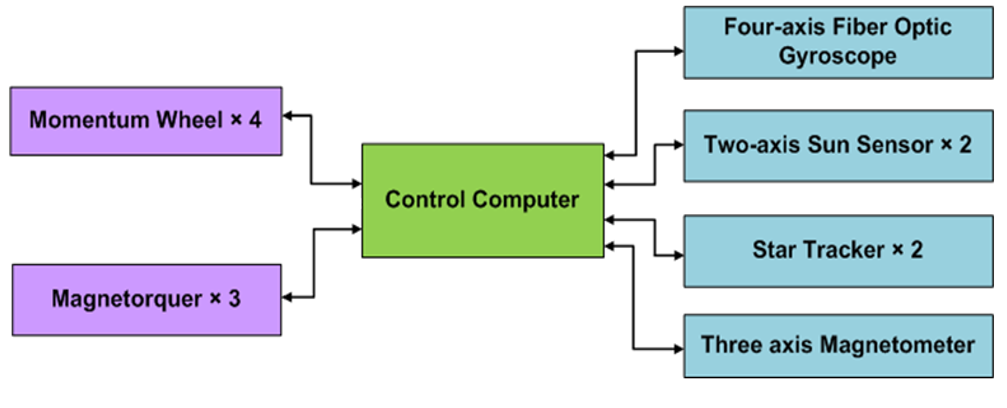
\includegraphics[width=.5\textwidth]{image/AOCS composition.PNG}
		\caption{ETRSS-1 satellite AOCS composition}
	\end{figure}
	\item Momentum wheel: Momentum wheels are nominally treated as a black box for missions that do not require precise pointing \cite{Wang2019AdaptiveMD} and are regarded as an ideal unit capable of producing the required control torque accurately, regardless of jitter or other disturbances.  Magnetic actuators can be used to reduce the torque required by the reaction wheel, allowing satellites to run their momentum wheels at a slower rotation speed in order to reduce jitter. ETRSS-1 AOCS subsystem employs FW-SR.090.0.1-1C momentum wheel as the primary maneuvering actuators and core devices for implementing zero-momentum control strategy. Furthermore, the actuators provide external torque to the ETRSS-1 satellite in order to achieve high attitude control performance and angular rate, as well as to construct the total angular momentum of the entire satellite in order to achieve zero angular momentum with four wheels. Earth satellite attitude control systems frequently use magnetic actuation, in which the mechanical torque required for attitude control is generated by the magnetic interaction between the geomagnetic field and on-board electromagnets or magnetic torquers \cite{Bhat2003ControllabilityOS}. ETRSS-1 momentum wheels X, Y, and Z are mounted orthogonally within their angular momentum vectors paralleled with respect to the +X, +Y, +Z axis of the satellite coordinates, while the momentum wheel S is mounted equi-angularly with the -X, -Y, -Z axis of the satellite coordinates. The wheel weighs 1kg, has a working speed of 6000rpm, a maximum moment output of 15 Nm, an angular momentum of 0.36 Nm/s, and a steady state power consumption of about 9W.
	\item Magnetic torquer: The magnetic torquer on the ETRSS-1 AOCS can provide controllable magnetic momentum change of the satellite by using the effect of the Earth's magnetic field. It is primarily used for unloading angular momentum and magnetic damping, and it can provide torque to reduce the speed of the momentum wheels from real-time to nominal speed. 
\end{enumerate}
\subsubsection{Spacecraft attitude dynamics}
The attitude dynamics of a spacecraft modeled as a rigid body rotating in space with fly wheels and an inertial matrix J whose origin is at the center of mass and whose reference frame is fixed to the satellite body could be described using Euler's equation of motion. 
\begin{equation}
	J\dot{\omega}(t) = -\omega(t) \times J\omega(t) + T_c(t) + T_d(t)
\end{equation}
where $\omega(t)$ is the angular velocity vector expressed in a body reference frame and J is the inertia matrix, such that $J = J^T$, and $T_c$, $T_d$ are, respectively, the control and disturbance torques acting on a satellite (caused by the space environment: light pressure, aerodynamic torque). The satellite's angular momentum is composed of the body angular momentum H and angular momentum h generated by momentum devices installed on the satellite, yielding
\begin{equation}
	\dot{H} = - \dot{h} + T_c + T_d
\end{equation}
and because the external torque affects the satellite's angular momentum, we have:
\begin{equation}
	H(t) = H(0) + h(0) - h(t) + \int_0^{t}T_cdt + \int_0^{t}T_ddt
\end{equation}
where $H(0)$ is the initial value of body angular momentum, $h(0)$ is the initial value angular momentum caused by momentum device, $\int_0^{t}T_cdt$ and $\int_0^{t}T_ddt$ are the external control angular momentum and external disturbing angular momentum respectively. As a result, solving attitude control problems becomes a matter of determining the values of $H(0)$ and $(0)$ while handling the external disturbing angular momentum, $H_d(t)$. Normally, we keep $h(0) =0$ which is called zero angular momentum control. Thus, in this case, $h(t)$ by momentum wheel and external control angular momentum, $H_c(t)$ by thruster and magnetic torquer have to deal with $H_d(t)$. Fig.3 depicts the on-orbit results of ETSS-1 attitude dynamics damping moment.
\begin{figure}
		\centering
		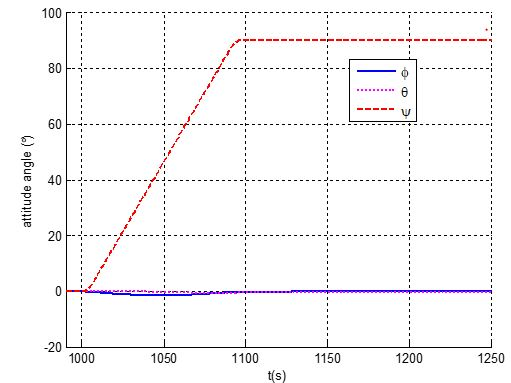
\includegraphics[width=1\linewidth]{image/attitude manuever }
		\caption{ ETRSS-1 90 degree attitude maneuver  maintaining mode}
\end{figure}
\subsection{Communication subsystem (TT$\&C$)}
The telemetry, tracking, and command (TT$\&$C) subsystem serves as an interface between the spacecraft and ground systems \cite{larson1992space}, allowing payload mission data and spacecraft housekeeping data to be sent from the spacecraft to operators and users at operation centers. The operator commands are also transmitted via this subsystem to the spacecarft in order to control it and operate the payload.  The ETRSS-1 satellite communication subsystem is primarily composed of three major components:
\begin{itemize}
	\item Transponder: ETRSS-1 TT$\&$C subsystem consists of two transponder A and B which are used to transmit telemetry data as well as receive and modulate up-link signals and output pulse code modulation signals to the on-board data handling system.
	\item GPS recievier: which is used to output position and orbit determination messages, broadcast the UTC time, and the power supply signal, which synchronizes the satellite time.
	\item Antenna system: which receives or transmits the telemetry and telecommand signal.
\end{itemize}
\subsection{Onboard data handling (OBDH)subsystem}
The on-board data handling subsystem performs two major functions \cite{larson1992space}.The ETRSS-1 OBDH subsystem is the satellite's electronic system's kernel, responsible for satellite onboard operations and information handling. It also receives telecommand and data blocks from ground stations and distributes them to spacecraft subsystems, as well as collects satellite telemetry data and transmits it to ground stations.  Overall, it receives, validates, decodes, and distributes commands to other spacecraft systems, as well as gathers, processes, and formats spacecraft housekeeping and mission data for downlink or use by an on-board computer. It often includes extra services like spacecraft timekeeping, computer health monitoring, and security interfaces. While command and data handling are generally different activities, combining them into a single subsystem provides an effective means of autonomous control of spacecraft functions. 
Fig. 5 depicts the composition layout of the ETRSS-1 onboard data handling subsystem.
\begin{figure}[hbt!]
	\centering
	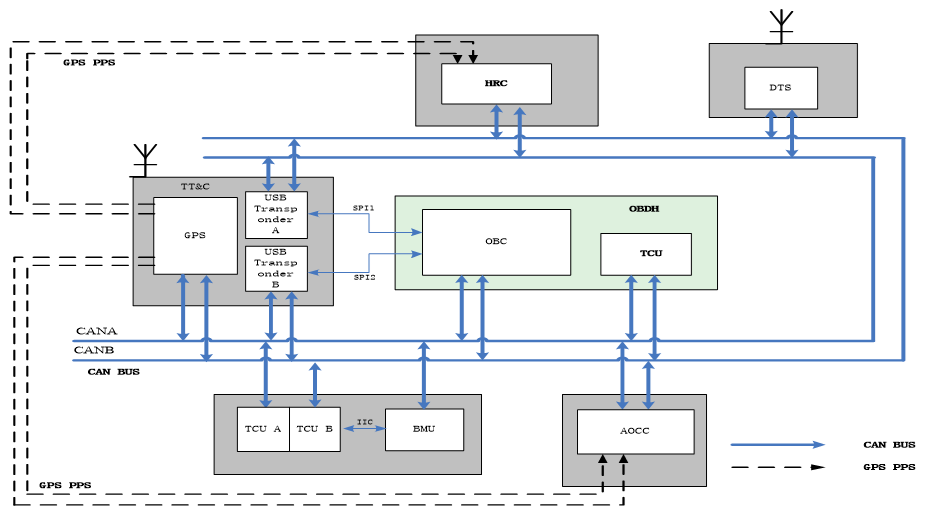
\includegraphics[width=.5\textwidth]{image/obdh}
	\caption{Schematic of the ETRSS-1's Onboard Data Handling Subsystem}
\end{figure}
\subsection{Electrical power supply subsystem (EPS)}
The electrical power subsystem provides, stores, distributes, and controls spacecraft electrical power \cite{larson1992space}. The ETRSS-1 power supply system generates, reserves, transforms, manages, and distributes power on the satellite.  Furthermore, the system converts light energy or chemical energy into electrical energy by a physical or chemical change, and it provides power supply and distribution for the platform and payloads during testing, launching, and orbiting. The ETRSS-1 spacecarft's electrical power supply subsystem is made up of three key components: a solar cell array, a battery, and a power control and distribution unit (PCDU). The entire solar-array is composed of several solar cells connected in series and parallel to obtain the appropriate voltage and current. The ETRSS-1 electrical power supply subsystem made use of a triple junction GaAs solar cell type and three solar panels, one for surface mounting and two for fixed solar wings, each with one panel. The overall area of the solar arrays that meet the power requirements is 0.70 $m^2$.  The subsystem's battery structure is built of 7 lithium-ion battery cells with improved power and energy density, a wider temperature range, higher charging efficiency, and bertter durability at a current total capacity of 10Ah.
\begin{figure*}[h!]
	\begin{subfigure}{.5\textwidth}
		\centering
		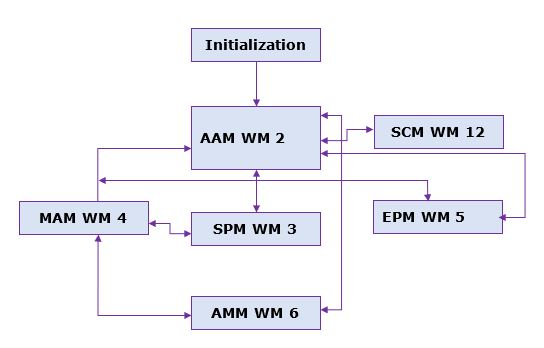
\includegraphics[width=.8\linewidth]{image/AOCS wm}
		\caption{The control and operation modes of AOCS}
		%\label{fig:my_label}
	\end{subfigure}%
	\begin{subfigure}{.5\textwidth}
		\centering
		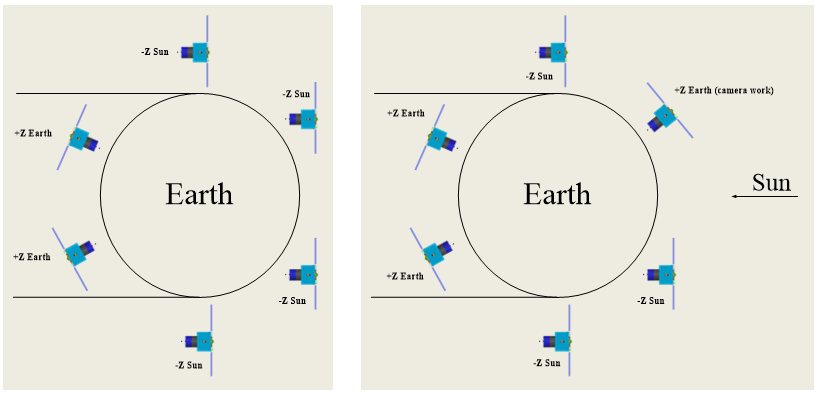
\includegraphics[width=.8\linewidth]{image/attitude control}
		\caption{ETRSS-1 attitude control and pointing schematics}
	\end{subfigure}
	\caption{The schematics of ETRSS-1 attitude control and working mode}
\end{figure*}
\subsection{Thermal control subsystem (TCS)}
The thermal control subsystem's function is to keep all spacecraft and payload components and subsystems within their allowable and specified temperature limits for each mission phase \cite{rotteveel2005thermal}.
\begin{table}[ht]
	\small
	\caption{Typical thermal requirements of ETRSS-1 spacecraft components} % title of Table
	\centering % used for centering table
	\scalebox{0.95}{
		\begin{tabular}{c c c c} % centered columns (4 columns)
			\hline\hline %inserts double horizontal lines
			Equipment& Operating& Survival \\ [0.5ex] % inserts table
			%heading
			\hline % inserts single horizontal line
			Electronics & - 15 C$^{\circ}$ $\sim$  50 C$^{\circ}$ & - 25 C$^{\circ}$ $\sim$ 60 C$^{\circ}$ \\ % inserting body of the table
			Battery &  10 C$^{\circ}$ $\sim$ 30 C$^{\circ}$ & 20 C$^{\circ}$ $\sim$ 40 C$^{\circ}$\\
			Antenna & - 90 C$^{\circ}$ $\sim$ 90 C$^{\circ}$ & - 110 C$^{\circ}$ $\sim$ 130 C$^{\circ}$\\
			Star sensors & - 30 C$^{\circ}$ $\sim$ 45 C$^{\circ}$ & - 40 C$^{\circ}$ $\sim$ 55 C$^{\circ}$\\
			Most platform units & - 15 C$^{\circ}$ $\sim$ 50 C$^{\circ}$ & - 25 C$^{\circ}$ $\sim$ 700 C$^{\circ}$\\
			Payload units & - 15 C$^{\circ}$ $\sim$ 50 C$^{\circ}$ & - 25 C$^{\circ}$ $\sim$ 700 C$^{\circ}$\\
			Momentum wheel & - 10 C$^{\circ}$ $\sim$ 45 C$^{\circ}$ & - 20 C$^{\circ}$ $\sim$ 55 C$^{\circ}$\\
			Structure & - 90 C$^{\circ}$ $\sim$ 90 C$^{\circ}$ & - 100 C$^{\circ}$ $\sim$ 100 C$^{\circ}$ \\ [1ex] % [1ex] adds vertical space
			\hline %inserts single line
		\end{tabular}
	}
	\label{table:nonlin} % is used to refer this table in the text
\end{table}
 There are two types of temperature limits \cite{larson1992space} that are typically defined: operational limits, which the component must adhere to while operating, and survival limits, which the component must adhere to at all times, even when not powered. In contrast to out-of-tolerance performance when operational limits are exceeded, exceeding survival temperature restrictions might result in irreversible device damage.  The ETRSS-1 thermal control subsystem expected to keep all of the equipment and structure within the temperature range requirements under all expected constraint circumstances.  Table 3 illustrates the typical needed ETRSS-1 component temperature ranges for representative spacecraft components. The thermal control of the ETRSS-1 system is comprised of up of copper plate, multi-layer insulation (MLI), OSR, SR107, SR107-ZK, heater, thermal grease, velcro, glue, ground material, and other components total weighing $\leq$ 3.5 kg.
\subsection{Data transmission subsystem (DTS)}
The ETRSS-1 DTS subsystem is a critical subsystem that receives data from the multi-spectral camera, compresses, replays, processes, and finally transmits it to the ground station at up to 100 Mbps. It also possesses the function of data formatting, recording, modulating and data transmission. It is made up of three major components: an integrated transmission machine, a phase array antenna, and a coaxial wire. The integrated transmission machine consists of a base band segment, an RF processing segment, and a power source segment. The phased-array antenna receives signals from the integrated transmission machine and transmits them to the ground station, whereas the coaxial cable transmits RF signals from the integrated transmission machine to the phased-array antenna.
\section{On-orbit performance analysis}
\subsection{AOCS's safe control mode of Operation}
To complete the imaging mission, ETRSS-1's AOCS collaborates with other subsystems and will use several command sequences to implement the cooperation by providing a satisfied attitude condition. The AOCS on the ETRSS-1 satellite operate in six modes: global attitude acquisition mode, sun pointing mode, maneuver mode, earth pointing mode, attitude maintaining mode, and stop control mode.
Global attitude acquisition mode employs a fiber optical gyroscope, a sun sensor, a magnetometer, a star sensor, and actuators such as a momentum wheel to reduce the satellite's angular velocity to the required range, as well as magnetic torques to stabilize the satellite after separation and drive the attitude close to nominal. Sun pointing mode is the satellite's normal operation mode, and the attitude determination scheme is "FOG with STS" or "FOG with magnetometer," in which the attitude is controlled by a momentum wheel and the redundant angular momentum is unloaded by magnetic torque. Maneuver mode is an interim mode that uses the estimation of FOG to implement attitude determination and momentum wheel to complete the attitude maneuver. The satellite operates in a three-axis zero-attitude earth-orientation mode, with attitude determination schemes comprised of a fiber optical gyro coupled with a star sensor or a fiber optical sensor coupled with a magnetometer. Attitude maintaining mode is followed by the maneuver mode to maintain the required attitude, roll angle for imaging, or yaw 90° for calibration. The satellite can enter the stop control mode autonomously or via ground station control. In this mode, the central control unit no longer works on attitude control and only performs measurement and orbit calculation, and the output of the actuators is ZERO. Figure 4 depicts the conditions for the ETRSS-1's attitude control and mode of operation, while Figure 5 depicts the attitude angle and its corresponding angular velocity from January 2020 to 2023. When the satellite is in Earth pointing mode and attitude maintaining mode, its roll, pitch, and yaw angle vary between -0.1$^{\circ}$ and +0.1$^{\circ}$. However, when in the earth pointing mode and attitude maintaining mode, the corresponding attitude angular velocity of the satellite, including the roll and pitch angular velocity, varies between -0.01$^{\circ}$/s and +0.01$^{\circ}$/s, while the yaw angular velocity varies between -0.1$^{\circ}$/s and +0.1$^{\circ}$/s.
\subsection{ETRSS-1 anomaly detection and management}
The space environment is hostile, and it is not a benign vacuum into which a thing can be placed and expected to function exactly as it did when developed and tested on Earth \cite{vampola1994analysis}.  Spacecraft cannot even be held in space for an extended period of time due to the severe degradation of surfaces and electronic components, as well as the various undesirable interactions that occur. Total dosage damage to mechanical and electrical components caused by the confined energetic particle environment, solar protons, and cosmic rays is a key category \cite{vampola1994analysis}. The fault detection and isolation functions at the component level act on sensor signals after low-pass filtering. Thus, defect identification is performed on the raw filtered sensor values and is based on statistical analysis of the incoming signal \cite{colagrossi2022fault}. These functions work on low-pass filtered data to ensure consistency of behavior between sensors with and without incorporated low-pass filtering. The complexity in detecting fault is related to the dynamical evolution of the nominal sensor signals along the spacecraft's generic attitude state, and the detection algorithms should be capable of identifying a variation that is not compatible with a realistic dynamical state of the spacecraft \cite{colagrossi2022fault}. In general, malfunctions are classified into four major categories based on their impact on the ETRSS-1 satellite in orbit, and measures to mitigate the impact of failures are covered in this section.
\begin{itemize}
	\item Category I-Catastrophic failure: This failure results in the loss of all or some functions, the failure of a task, a reduction in lifetime, property damage, or personnel loss. For example attitude control and power loss.  It must deal with it swiftly, or else the satellite may fail. Catastrophic failure typically occurs during the active phase or two circles prior to orbit.
	\item Category II-Critical failure: This failure causes the loss of subsystem functions, interface payload tasks, equipment function degnertaes or loss, and the spacecraft may lose some functions following treatments. For example, a solar array invalidated/attitude abnormal/equipment reconfiguration can be recovered with human intervention, but control accuracy will be reduced/payload function will be compromised, or date downlink function will not be restored completely. It should be addressed in the current orbit, and if that is not possible, it should be addressed in the following orbit circle.	
	\item Category III-Minor failure: This failure comprises major function degeneration or loss of equipment. After treatment, the satellite may lose some backup functions, but the subystem will not be affected. For example, an OBC backup failure and a drop in solar array output. It should be countermeasured based on the investigation of telemetry data to determine the cause.
	\item Category IV-Slight failure: This failure has no effect on the main function of the subsystem. For example, switching from main to backup work state, SSE-caused sub-computer reset, and it should be countermeasured based on telemetry data analysis to determine the failure reason.
\end{itemize}
\begin{figure*}[h!]
	\begin{subfigure}{.5\textwidth}
		\centering
		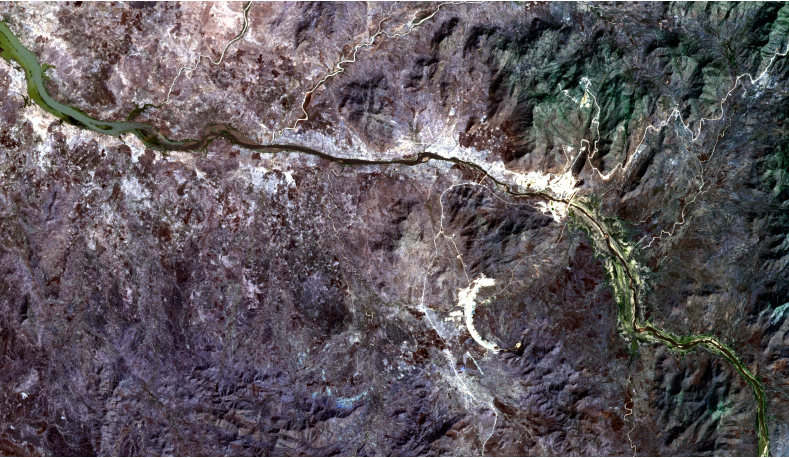
\includegraphics[width=.8\linewidth]{image/GERD.PNG}
		\caption{ETRSS-1 Grand Ethiopian Renaissance Dam}
		%\label{fig:my_label}
	\end{subfigure}%
	\begin{subfigure}{.5\textwidth}
		\centering
		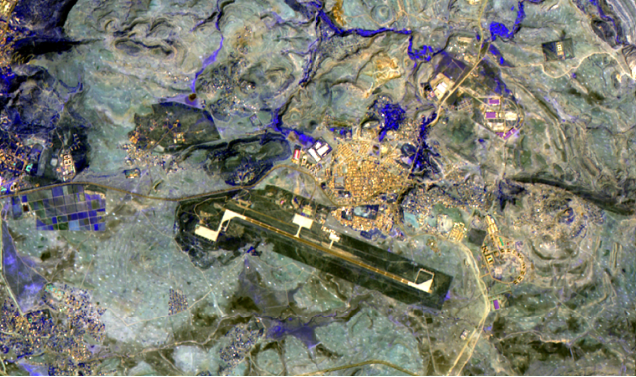
\includegraphics[width=.8\linewidth]{image/mek}
		\caption{ETRSS-1 Mekele Airport, Ethiopia}
	\end{subfigure}
	\begin{subfigure}{.5\textwidth}
		\centering
		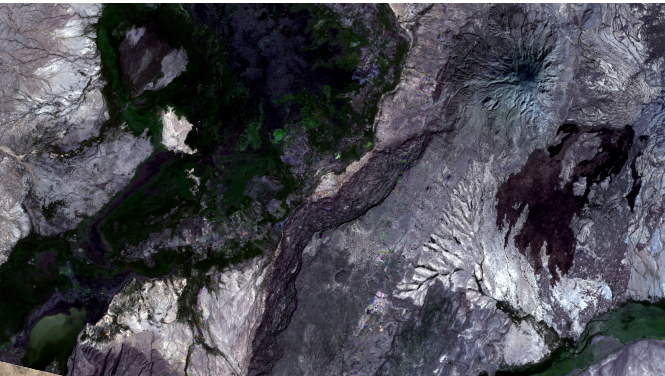
\includegraphics[width=.8\linewidth]{image/afar}
		\caption{ETRSS-1 Afar, Rassa National park}
	\end{subfigure}
	\begin{subfigure}{.5\textwidth}
		\centering
		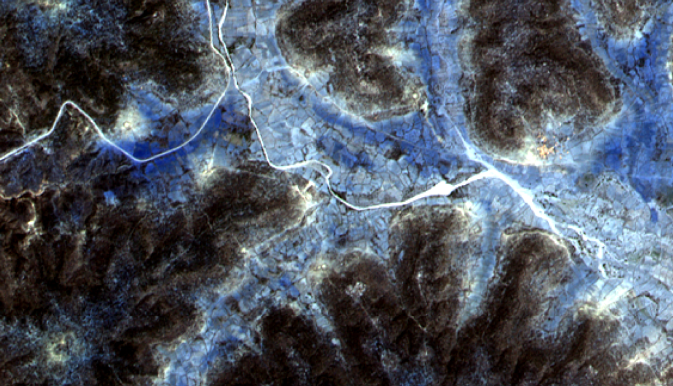
\includegraphics[width=.8\linewidth]{image/so}
		\caption{ETRSS-1 Somali around Elkere}
	\end{subfigure}
	\caption{Multi-spectral imagery data acquired by ETRSS-1 optical payload}
\end{figure*}
During the satellite's operation, two major problems were discovered: the spacecraft entered safe mode, impairing the imaging mission, and the ground station was stacked for some time, making contact with the spacecraft impossible. During safe mode, the spacecraft's solar panel is pointed toward the sun, all other subsystems are working, and the payload is shut off. Furthermore, critical telecommands have been sent to the spacecraft in order to clear the faults, and the on-board data handling subsystem monitors the required parameters and operates the satellite's safe mode. In fact, the on-board data handling system is mainly in charge of system-level FDIR to maintain the satellite system's safety, and it directly or indirectly checks battery voltage, battery temperature, AOCS mode, and the communication status of various equipment. Critical telecommands (such as the state of the power supply system and the AOCS) are provided to the spacecraft during anomaly detection and are monitored by the on-board data handling subsystem. When the essential telecommands are unsuccessful, the on-board data handling system sends a safe command sequence, such as turning off the payload, to guarantee that the satellite's energy is preserved securely. When safe mode occurs, the safe mode execute counter changes, allowing mission operators to cope with the situation.
\subsection{Optical multispectral camera imaging}
Optical imaging has been one of the most on-orbit missions of the ETRSS-1 microsatellite, due mainly to the satellite's good attitude performance. ETRSS-1 is equipped with a reinforced multispectral camera module for optical imaging, with a Ground Sampling Distance (GSD) of 13.4m at an orbit altitude of 628km and a swath of 80km. The primary purpose of the ETRSS-1 optical camera system is to take images in nadir or roll maneuver, transmit the imagery data to the digital transmission system (DTS), enter into safe mode automatically after 15 minutes of uninterrupted image taking, and perform imaging radiation calibration to the ground when the spacecraft yaws 90$^{\circ}$. The ETRSS-1 optical camera payload is made up of two major parts: the secondary power and the camera main body system, which includes the optical lens, light shield, focal plane, and process components.   The secondary power receives primary power from the spacecraft (23 $\sim$ 29V) and transfers primary power to the focal plane and video processor. Furthermore, Figure 6 depicts the optical imagery captured by ETRSS-1 at various points in time and locations, including the Grand Ethiopian Renaissance Dam construction image. The image shows that the multispectral camera can capture the Earth, proving that the AOCS for ETRSS-1 is suitable and effective.
\subsection{End-of-life (EOL) disposal}
There a need to control a rise in the number of space junk, or non-functioning human-made objects in low earth orbit, which will have long-term implications on satellite operation. Responsible exit from Low Earth Orbit (LEO) is one of the most significant actions that may be taken to limit the growth of debris in that region of space in order to reduce explosions and breakups, prevent collisions of space objects, and dispose of space hardware at end-of-mission \cite{ailor2010spacecraft}. Furthermore, for spacecraft in low-Earth orbit (LEO), atmospheric disposal within 25 years of end-of-life (EOL) is regarded as the most effective approach of achieving orbital debris mitigation standards. The residual atmosphere remaining at orbital altitudes causes orbital decay, which will naturally de-orbit a spacecraft within the stipulated 25-year time-frame at sufficiently low orbital altitudes \cite{rhatigan2020drag}. The Ethiopian remote sensing satellite weighing 65kg with an average windward area of 0.354 $m^2$ and orbital altitude of 628 km will decay continuously, and the satellite will reentry into the atmosphere ($\leq$ 100km) within 25 years.  Fig. 7 depicts the orbital decay of the Ethiopian remote sensing satellite.
\begin{figure}[!htb]
	\centering
	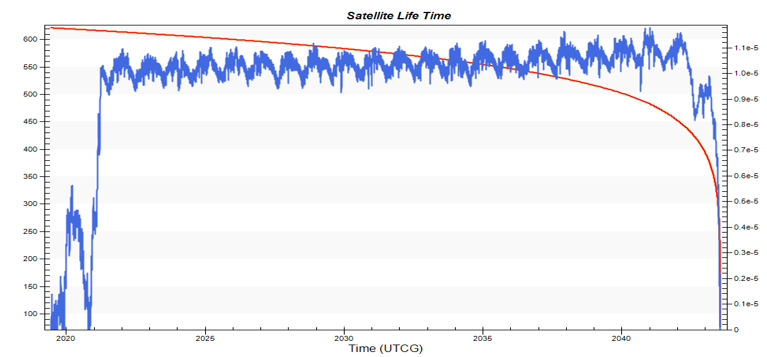
\includegraphics[width=.9\linewidth]{image/Etrss-1 life time}
	\caption{Ethiopian remote satellite orbital decay }
	%\label{fig:my_label}
\end{figure}%bt
Furthermore, ETRSS-1 spacecraft experience natural orbital decay due to atmospheric drag over time. This atmospheric drag causes the spacecraft's orbital altitude to gradually decrease over time. As the spacecraft descends into a lower orbit, the atmospheric density increases, resulting in greater drag forces. This drag eventually diminishes the spacecraft's speed and energy, causing its orbit to decay more. It is apparent that the rate of orbital decay is affected by a number of elements, including the spacecraft's mass, shape, and cross-sectional area, as well as the air conditions at its altitude. Larger and more massive spacecraft endure increased atmospheric drag and degrade at a faster rate. 
\section{Conclusion}
The ETRSS-1 satellite has been in orbit for more than three years, operating from a sun-synchronous orbit at an altitude of 628 kilometers, and has completed all missions successfully by providing imagery data via a ground control station facility located at Entoto. 
The investigation of ETRSS-1 on-orbit performance and anomaly management provides vital insights into the satellite's operating capabilities and the actions used to resolve any unexpected events or malfunctions. The study shed light on the satellite's health, condition, and general operation by evaluating telemetry data and assessing key subsystems such as attitude control, communication, power, and thermal management. For instance, according to the satellite's original telemetry data, the attitude angle of the satellite changes between -180$^{\circ}$ and +180$^{\circ}$ when in operational modes other than Attitude Acquisition Mode and Earth Pointing Mode.  \\
The analysis revealed that ETRSS-1 accomplished satisfactorily on-orbit, meeting the predicted requirements and effectively carrying out its intended functions. While some minor anomalies were observed during its operating lifetime, the anomaly management process adopted by the mission operators was successful in identifying, diagnosing, and resolving these issues in a timely way. This proactive strategy guaranteed that the satellite's mission objectives were disrupted as little as possible.\\
Furthermore, the investigation' findings gave useful insights into ETRSS-1's performance, allowing for changes in operational processes and anomaly reaction strategies. The insights obtained from this analysis can be applied to future satellite missions, resulting in improved mission planning, operational efficiency, and anomaly handling techniques.\\
Overall, the ETRSS-1 on-orbit performance and anomaly management investigation has offered a thorough understanding of the satellite's behavior in orbit. The successful control of anomalies, as well as the overall performance of the satellite, confirmed the mission's design and operational plans. This study will be used as a reference for future satellite missions, offering significant insights into the hurdles encountered during on-orbit operations as well as the successful strategies implemented to assure mission success.
\section*{CRediT authorship contribution }
\textbf{Gadisa Dinaol }: Conceptualization,  Writing - Original draft, Methodology, Data curation, Writing -review and editing, and Visualization.
\section*{Acknowledgment}
The authors would like to thank the ETRSS-1 designer and operator teams, as well as the engineers at China DFH satellite Co.Ltd, for their unflinching support throughout the mission.
\section*{Declaration of competing interest}
The authors declare that they have no known competing financial interests or personal relationships that could appear to have influenced the work described in this paper.
\section*{Funding sources}
This study received no specific funding from public, commercial, or non-profit funding agencies.
%\printcredits
\bibliographystyle{unsrtnat} 
\bibliography{sample}

%% else use the following coding to input the bibitems directly in the
%% TeX file.

%\begin{thebibliography}{00}

%% \bibitem[Author(year)]{label}
%% Text of bibliographic item

%\bibitem[ ()]{}

%\end{thebibliography}
\end{document}

